% !Rnw root = learnR.Rnw

%% ---preamble.tex----%% 
%% maxwidth is the original width if it is less than linewidth
%% otherwise use linewidth (to make sure the graphics do not exceed the margin)
\makeatletter
\def\maxwidth{ %
  \ifdim\Gin@nat@width>\linewidth
    \linewidth
  \else
    \Gin@nat@width
  \fi
}
\makeatother

\definecolor{fgcolor}{rgb}{0.345, 0.345, 0.345}

\definecolor{shadecolor}{rgb}{.97, .97, .97}
\definecolor{messagecolor}{rgb}{0, 0, 0}
\definecolor{warningcolor}{rgb}{1, 0, 1}
\definecolor{errorcolor}{rgb}{1, 0, 0}






%\noindent
\fbox{\parbox{\textwidth}{
\vspace*{-2pt}

\begin{tabular}{ll}
Scatterplot & Scatterplot matrices can give useful insights on\\
matrices    & data that will be used for regression or related\\
 &  calculations.\\[6pt]
Transformation & Data often require transformation prior to entry\\
& into a regression model.\\[6pt]
Model  & Fitting a regression or other such model gives,\\
objects     & in the first place, a model object.\\[6pt]
Generic & \txtt{plot()}, \txtt{print()} and \txtt{summary()} are examples\\
functions & of {\em generic} functions.  With a dataframe as \\
          & argument \txtt{plot()} gives a scatterplot matrix.\\
          & With an \txtt{lm} object, it gives diagnostic plots.\\[6pt]
Extractor & Use an extractor function to extract output from\\
function  & a model object. Extractor fucntions are {\em generic}\\
          & functions\\[6pt]
List objects & An \txtt{lm} model object is a list object. Lists are\\
 & used extensively in R.\\
\end{tabular}
}}
\vspace*{8pt}

\marginnote[12pt]{Issues that will be noted include the use
  of {\em generic} functions such as \txtt{plot()} and \txtt{print()},
  the way that regression model objects are structured, and the use of
  extractor functions to extract information from model objects.}
This chapter will use examples to illustrate common issues in the
exploration of data and the fitting of regression models.  It will
round out the discussion of Chapters \ref{ch:getStart} and
\ref{ch:workenv} by adding some further important technical details.

\subsection*{Notation, when referring to datasets}

Data will be used that is taken from several different R packages.
The notation \txtt{MASS::mammals}, which can be used in code as well
as in the textual description, makes it clear that the dataset
\txtt{mammals} that is required is from the {\em MASS} package.
Should another attached package happen to have a dataset
\txtt{mammals}, there is no risk of confusion.

\section{Science, statistics, and R}

How does statistical analysis fit into the wider scientific
enterprise? While not a central focus of the present notes, 
the issues that will now be noted are too important to be
ignored.

The R system is an enabler that allows users to do effective
data analysis, and much else besides.  These notes hint at
its scope, primarily for data manipulation, for data analysis,
and for graphics.  Note, however, the chapters on map overlays
and on text mining --- these extend into areas that would not
ordinarily be described as "data analysis".

For the purposes of this next, the terms "data science" and
"statistics" are different names for an endeavour whose concern
is to extract meaning from data, leading for example to results
that might be reported in a scientific paper, or that might form
the basis for a business or government policy.  Statistical
issues and ideas are fundamental to any use of data to make
generalizations that extend beyond the particular data that
have been collected, or that are otherwise available.  They are
fundamental, in that sense, to any scientific use of data.
It is, at the same time, important to acknowledge that there
are strict limits on what statistical analysis can achieve.
Statistical analysis is a partner to, and not a substitute
for, robust scientific processes.  The use of experimental data
provides the simplest context in which to explore this point
further.

For experimental work, over and above what may emerge from a
statistical analsysis, the demand is that results be replicable.
Laboratory studies have repeatedly shown shown that drinking
regular caffeinated coffee increases blood pressure, though
with minimal long term effects.\footnote{\citet{green_kirby_suls_1996}
}  It is accepted that there is
this effect, not from the statistical analysis of results from
any individual trial, but because the effect has been demonstrated
in repeated trials.  The role of statistical analysis has been:
\begin{enumerate}
\tightlist
\item to demonstrate that, collating the evidence from repeated
trials, the effect does appear real; 
\item to assess the magnitude of the effect.
\end{enumerate}

Worldwide, hundreds of thousands of randomised trials are
conducted annually.  What do they tell us?  In clinical medicine,
follow-up trials are common, and clear conclusions will often
emerge from the careful collation of evidence that, in important
cases, is likely to follow.  In many other areas follow-up trials
have until recently been uncommon. This is now changing, and for
good reason.  Independent replication of the experimental process
provides checks on the total experimental process, including the
statistical analysis.  It is unlikely that the same mistakes in
experimental procedure and/or statistical analysis will be repeated.

Papers that had a key role in getting attention to reproducibility
concerns have been \citet{prinz2011believe} and 
\citep{begley2012drug}, the first (6 out of 53 "landmark" studies
reproduced)  relating to drug trials, and the second (19 out of 65 
"seminal" studies) to cancer drug trials.  Since those studies
appeared, results have appeared from systematic attempts to
reproduce  published work in psychology (around 40\%), in
laboratory economics (11 of 18), and in social science (12 of 18).
These replication rates are so low, in these areas, that they make
nonsense of citations to published individual trial results as
evidence that a claimed effect has been scientifically demonstrated.

Many of the problems that these studies identify extend, also,
into research and associated analyses that works with observational
data.  In any attempt to draw hard conclusions from observational
data, in a case where the aim is to compare two groups, there are
certain to be many more differences than the difference that is
of interest.  One application of regression methods is to do
"covariate adjustments".  The limitations of such an approach are
not as widely understood as they should be. There has
to be confidence that all relevant covariates are accounted for,
that they are measured with adequate accuracy, and that the form
of the adjustment (e.g., $x$, or $\log(x)$, or $x^2$) is close
to correct.

In a hard-hitting paper titled "Cargo-cult statistics and
scientific crisis", \citet{stark_saltelli_2018} comment,
quoting also from \citet{edwards_roy_2017}:
\begin{quote}
While some argue that there is no crisis (or at least not a systemic problem), bad incentives, bad scientific practices, outdated methods of vetting and disseminating results, and techno-science appear to be producing misleading and incorrect results. This might produce crisis of biblical proportions: as Edwards and Roy write: ``If a critical mass of scientists become untrustworthy, a tipping point is possible in which the scientific enterprise itself becomes inherently corrupt and public trust is lost, risking a new dark age with devastating consequences to humanity.''
\end{quote}
Statistical issues are then front and central in what many are identifying
as a crisis, but are not the whole story. The crisis is one that
scientists and statisticians need to tackle in partnership.

In a paper that deserves much more attention than it has received,
\citep{tukey_1997}, John W Tukey
argued that, as part of the process of fitting a model and forming a
conclusion, there should be  incisive and informed critique of the data
used, of the model, and of the inferences made. It is important that
analysts search out available information about the processes that
generated the data, and consider critically how this may affect the
reliance placed on it. Other specific types of challenge (this list is
longer than Tukey's) may include:
\begin{itemize}
\tightlist
\item For experiments, is the design open to criticism?
\item Look for biases in processes that generated the data.
\item Look for inadequacies in laboratory procedure.
\item Use all relevant graphical or other summary checks to
critique the model that underpins the analysis.
\item Where possible, check the performance of the model on
test data that reflects the manner of use of results.
(If for example predictions are made that will be applied a
year into the future, check how predictions made a year
ahead panned out for historical data.)
\item For experimental data, have the work replicated
independently by another research group, from generation of
data through to analysis.
\end{itemize}
Exposure to diverse challenges will build (or destroy!) confidence
in model-based inferences. We should trust those results that have
withstood thorough and informed challenge. 

\subsection*{Where does R fit in?}

R clearly has a huge range of abilities for manipulating data, fitting
and checking statistical models, and for using graphs and tables to
present results.  More than this, it has extensive reproducible
reporting abilities that can be used to allow others to repeat the
data manipulation, analysis, and steps in the processing of output
that have led to an eventual paper or report.  A file is provided
that mixes code with the text for the eventual document, and that
is then processed ("woven" or "knitted") to provide the final
document, complete with analysis output, tables, graphs, and code
(if any) that is to be included in the final document.  This makes
it straightforward for referees, or for anyone with an interest in 
the work, to check the analysis and/or try modifications.
The publication of data and code is an important step on the way
to making results more open and transparent, and encouraging 
informed critique.


\section{The Uses of Scatterplots}

\begin{Schunk}
\begin{Sinput}
## Below, the dataset MASS::mammals will be required
library(MASS, quietly=TRUE)
\end{Sinput}
\end{Schunk}

\subsection{Transformation to an appropriate scale}

\marginnote{Among other issues, is there a wide enough spread
of distinct values that data can be treated as continuous.}
A first step is to elicit basic information on the columns in the
data, including information on relationships between explanatory
variables.  Is it desirable to transform one or more variables?

Transformations are helpful that ensure, if possible, that:
\begin{itemizz}
\item All columns have a distribution that is reasonably well spread
  out over the whole range of values, i.e., it is unsatisfactory to
  have most values squashed together at one end of the range, with a
  small number of very small or very large values occupying the
  remaining part of the range.
  \item Relationships between columns are roughly linear.
  \item the scatter about any relationship is similar across the whole
range of values.
\end{itemizz}
It may happen that the one transformation, often a logarithmic
transformation, will achieve all these at the same time.

The scatterplot in Figure \ref{fig:Animals}A, showing data from the
dataset \txtt{MASS::mammals}, is is an extreme version of the
common situation where positive (or non-zero) values are squashed
together in the lower part of the range, with a tail out to the right.
Such a distribution is said to be ``skewed to the right''.

Code for Figure \ref{fig:Animals}A
\begin{Schunk}
\begin{Sinput}
plot(brain ~ body, data=mammals)
mtext(side=3, line=0.5, adj=0,
      "A: Unlogged data", cex=1.1)
\end{Sinput}
\end{Schunk}

\begin{marginfigure}
\begin{Schunk}


\centerline{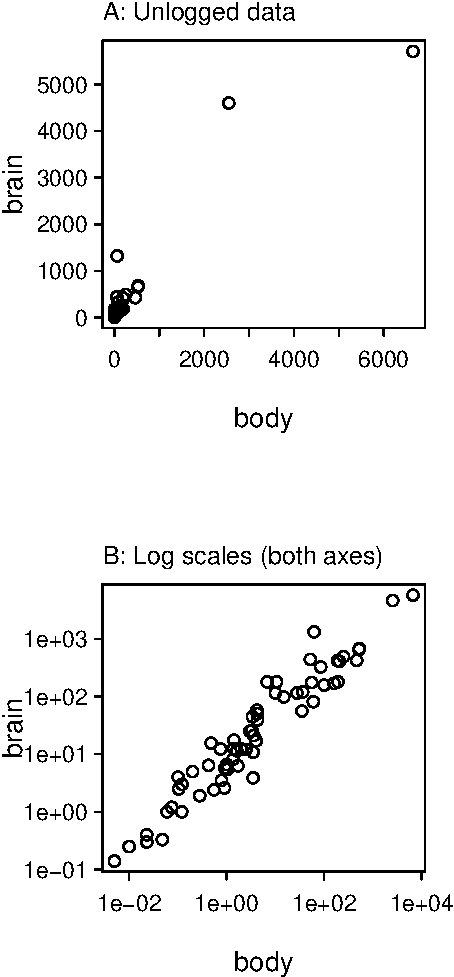
\includegraphics[width=\textwidth]{figs/03-bbAB-1} }

\end{Schunk}
\caption{Brain weight (g) versus Body weight (kg), for 62 species of mammal.
Panel A plots the unlogged data, while Panel B has log scales for
both axes, but with axis labels in the original (unlogged) units.
  \label{fig:Animals}}
\end{marginfigure}

Figure \ref{fig:Animals}B shows the scatterplot for the logged data.
Code for Figure \ref{fig:Animals}B is:
\begin{Schunk}
\begin{Sinput}
plot(brain ~ body, data=mammals, log="xy")
mtext(side=3, line=0.5, adj=0,
      "B: Log scales (both axes)", cex=1.1)
\end{Sinput}
\end{Schunk}

Where, as in Figure \ref{fig:Animals}A, values are concentrated at one
end of the range, the small number (perhaps one or two) of values that
lie at the other end of the range will, in a straight line regression
with that column as the only explanatory variable, be a leverage
point.  When it is one explanatory variable among several, those
values will have an overly large say in determining the coefficient
for that variable.

As happened here, a logarithmic transformation will often remove much
or all of the skew.  Also, as happened here, such transformations often
bring the added bonus that relationships between the resulting
variables are approximately linear.

\subsection{The Uses of Scatterplot Matrices}\label{sec:spm}

Subsequent chapters will make extensive use of scatterplot matrices.
A scatterplot matrix plots every column against every other column,
with the result in the layout used for correlation matrices.  Figure
\ref{fig:trees} shows a scatterplot matrix for the
\txtt{datasets::trees} dataset.  \marginnote[-24pt]{The
  \margtt{datasets} package is, in an off-the-shelf installation,
  attached when R starts.}

\begin{figure*}
\vspace*{-6pt}

\begin{minipage}[c]{0.55\linewidth}
\fbox{\parbox{\textwidth}{{\bf Interpreting Scatterplot Matrices:}\\[4pt]
For identifying the axes for each panel
\begin{itemizz}
\item[-] look across the row to the diagonal to identify the variable on
 the vertical axis.
\item[-] look up or down the column to the diagonal for the
  variable on the horizontal axis.
\end{itemizz}
Each below diagonal panel is the mirror image of the
corresponding above diagonal panel.
}}
\vspace*{6pt}

\begin{Schunk}
\begin{Sinput}
## Code used for the plot
plot(trees, cex.labels=1.5)
  # Calls pairs(trees)
\end{Sinput}
\end{Schunk}
\end{minipage}
\begin{minipage}[c]{0.465\linewidth}
\begin{Schunk}


\centerline{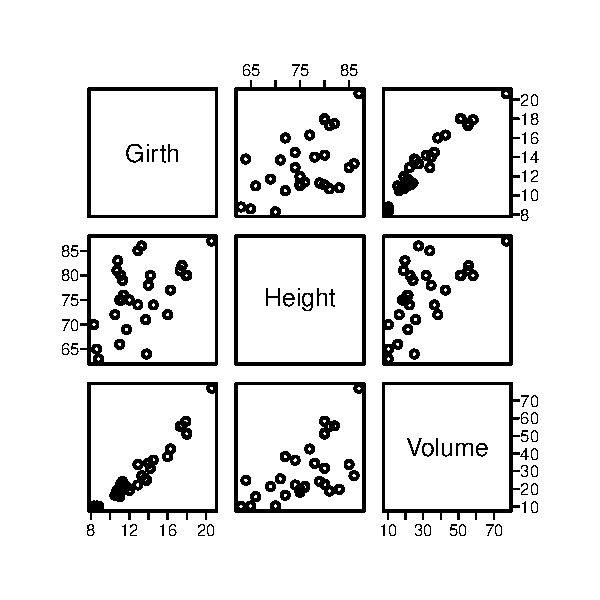
\includegraphics[width=\textwidth]{figs/03-plot-trees-1} }

\end{Schunk}
\vspace*{-15pt}

\end{minipage}
\caption{Scatterplot matrix for the \txtt{trees} data, obtained
  using the default \txtt{plot()} method for data frames.  The
  scatterplot matrix is a graphical counterpart of the correlation
  matrix.\label{fig:trees}}
\end{figure*}

Notice that \txtt{plot()}, called with the dataframe \txtt{trees},
has in turn called the plot method for a data frame, i.e.,
it has called \txtt{plot.data.frame()} which has in turn called
the function \txtt{pairs()}.

The scatterplot matrix may be examined, if there are enough
points, for evidence of:
\begin{enumerate}
  \marginnote[18pt]{The scatterplot matrix is best used as an initial
    coarse screening device. Skewness in the individual distributions
    is better checked using plots of density estimates.}
\item Strong clustering in the data, and/or
obvious outliers;
\item Clear non-linear relationships, so that a
correlation will underestimate the strength of any relationship;
\item Severely skewed distributions, so that the correlation is a biased
measure of the strength of relationship.
\end{enumerate}

\section{World record times for track and field events}\label{sec:wr}

The first example is for world track and road record times,
\marginnote{Note also the use of these data in the exercise at the end
  of Chapter 2 (Section \ref{ss:ch2ex})} as at 9th August 2006.  Data,
copied down from the web page
\url{http://www.gbrathletics.com/wrec.htm}, are in the dataset
\txtt{DAAG::worldRecords}.

\subsection*{Data exploration}
First, use \txtt{str()} to get information on the data frame columns:

\begin{Schunk}
\begin{Sinput}
library(DAAG, quietly=TRUE)
\end{Sinput}
\end{Schunk}

\begin{fullwidth}
\begin{Schunk}
\begin{Sinput}
str(worldRecords, vec.len=3)
\end{Sinput}
\begin{Soutput}
'data.frame':	40 obs. of  5 variables:
 $ Distance   : num  0.1 0.15 0.2 0.3 0.4 0.5 0.6 0.8 ...
 $ roadORtrack: Factor w/ 2 levels "road","track": 2 2 2 2 2 2 2 2 ...
 $ Place      : chr  "Athens" "Cassino" "Atlanta" ...
 $ Time       : num  0.163 0.247 0.322 0.514 ...
 $ Date       : Date, format: "2005-06-14" "1983-05-22" ...
\end{Soutput}
\end{Schunk}
\end{fullwidth}
%$

Distinguishing points for track events from those for road events is
easiest if we use lattice graphics, as in Figure \ref{fig:wrnolog}.

\begin{Schunk}
\begin{Sinput}
## Code
library(lattice)
xyplot(Time ~ Distance, scales=list(tck=0.5),
       groups=roadORtrack, data=worldRecords,
       auto.key=list(columns=2), aspect=1)
## On a a colour device the default is to use
## different colours, not different symbols,
## to distinguish groups.
\end{Sinput}
\end{Schunk}

\begin{marginfigure}
\begin{Schunk}


\centerline{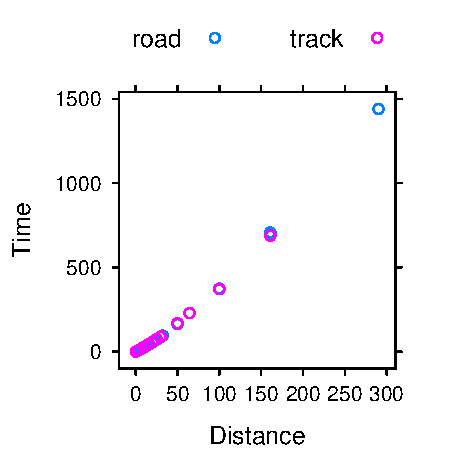
\includegraphics[width=0.98\textwidth]{figs/03-trackVSroad-1} }

\end{Schunk}
\caption{World record times versus distance, for field and road
  events.\label{fig:wrnolog}}
\end{marginfigure}

Clearly increases in \txtt{Time} are not proportional to increases in
\txtt{Distance}.  Indeed, such a model does not make sense; velocity
decreases as the length of the race increases.  Proportionality when
logarithmic scales are used for the two variables does make sense.

Figure \ref{fig:wrlog} uses logarithmic scales on both axes.  The two
panels differ only in the labeling of the scales.  The left panel uses
labels on scales of $\log_e$, while the right panel has labels in the
orginal units.  Notice the use of
\txtt{auto.key} to obtain a key.

\begin{figure}
\begin{Schunk}


\centerline{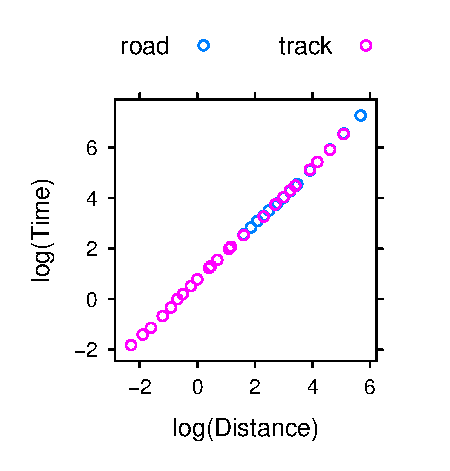
\includegraphics[width=0.47\textwidth]{figs/03-wrTimesAB-1} 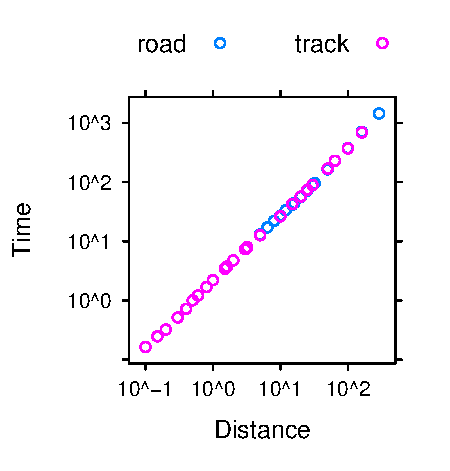
\includegraphics[width=0.47\textwidth]{figs/03-wrTimesAB-2} }

\end{Schunk}
\caption{World record times versus distance, for field and road
  events, using logarithmic scales.  The left panel uses labels on
  scales of $\log_e$, while in the right panel, labeling is in the
  orginal units, expressed as powers of 10.}
\label{fig:wrlog}
\end{figure}

\begin{Schunk}
\begin{Sinput}
## Code for Left panel
xyplot(log(Time) ~ log(Distance),
       groups=roadORtrack, data=worldRecords,
       scales=list(tck=0.5),
       auto.key=list(columns=2), aspect=1)
## Right panel
xyplot(Time ~ Distance, groups=roadORtrack,
       data=worldRecords,
       scales=list(log=10, tck=0.5),
       auto.key=list(columns=2), aspect=1)
\end{Sinput}
\end{Schunk}
\vspace*{-9pt}

\subsection*{Fitting a regression line}

The plots suggest that a line is a good fit.  Note however that the data span a
huge range of distances.  The ratio of longest to shortest distance is
almost 3000:1. Departures from the line are of the order of 15\% at
the upper end of the range, but are so small relative to
this huge range that they are not obvious.

The following \marginnote{The name \margtt{lm} is a mnemonic for
  {\underline{l}}inear {\underline{m}}odel.}  uses the function
\txtt{lm()} to fit a straight line fit to the logged data,
then extracting the regression coefficients:
\marginnote[1.0cm]{The equation gives predicted times:
\begin{eqnarray*}
\widehat{\mbox{Time}} &=& e^{0.7316} \times \mbox{Distance}^{1.1248}\\
&=& 2.08 \times \mbox{Distance}^{1.1248}
\end{eqnarray*}
This implies, as would be expected, that kilometers per minute
increase with increasing distance. Fitting a line to points that are
on a log scale thus allows an immediate interpretation.}
\begin{Schunk}
\begin{Sinput}
worldrec.lm <- lm(log(Time) ~ log(Distance),
                  data=worldRecords)
coef(worldrec.lm)
\end{Sinput}
\begin{Soutput}
  (Intercept) log(Distance) 
       0.7316        1.1248 
\end{Soutput}
\end{Schunk}
There is no difference that can be detected visually between the track
races and the road races.  Careful analysis will in fact find no
difference.

\subsection{Summary information from model objects}\label{ss:sum-modobj}
In order to avoid recalculation of the model information
\marginnote{The name \txtt{worldrec.lm} is used to indicate
that this is an \margtt{lm} object, with data from \txtt{worldRecords}.
Use any name that seems helpful!}
each time that some different information is required, we store the
result from the \txtt{lm()} calculation in the model object
\txtt{worldrec.lm}.

\begin{marginfigure}
Plot points; add line:
\begin{Schunk}
\begin{Sinput}
plot(log(Time) ~ log(Distance),
     data = worldRecords)
abline(worldrec.lm)
\end{Sinput}
\end{Schunk}
\end{marginfigure}
Note that the function \txtt{abline()} can be used
  with the model object as argument to add a line to the plot of
  \txtt{log(Time)} against \txtt{log(Distance)}.

\subsection*{Diagnostic plots}

Insight into the adequacy of the line 
\marginnote{By default, there are four ``diagnostic'' plots.}
can be obtained by examining the
``diagnostic'' plots, obtained by ``plotting'' the model object.
Figure \ref{fig:wr-diag} following shows the first and last of the default
plots:
\begin{Schunk}
\begin{Sinput}
## Code
plot(worldrec.lm, which=c(1,5),
     sub.caption=rep("",2))
\end{Sinput}
\end{Schunk}

\begin{figure}
\begin{Schunk}


\centerline{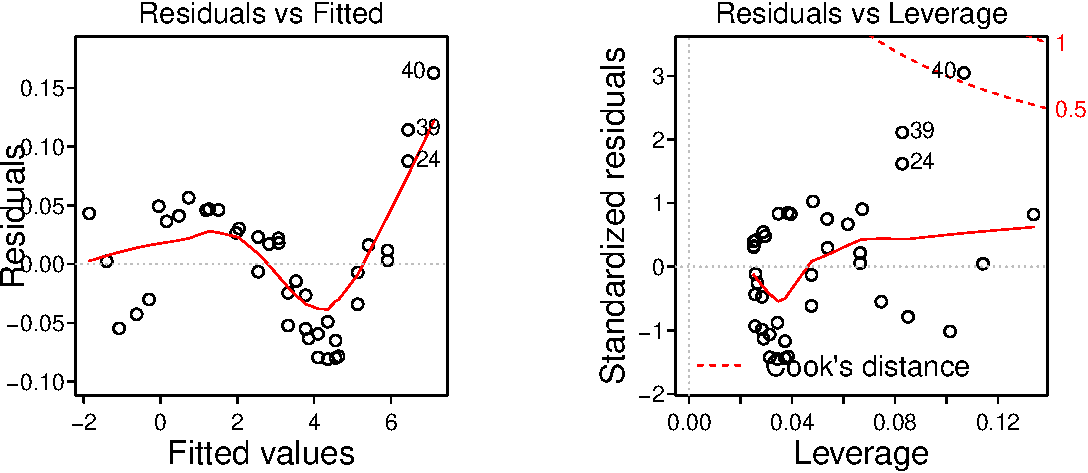
\includegraphics[width=\textwidth]{figs/03-diag12-1} }

\end{Schunk}
      \caption{First and last of the default diagnostic plots, from the
        linear model for log(record time) versus log(distance), for
        field and road events.}
\label{fig:wr-diag}
\setfloatalignment{t}% forces caption to be top-aligned
\end{figure}

Panel A is designed
to give an indication whether the relationship really is linear, or
whether there is some further systematic component that should perhaps
be modeled.  It does show systematic differences from a line.

The largest difference is more than a 15\% difference.\sidenote{A
  difference of 0.05 on a scale of $\log_e$ translates to a difference
  of just over 5\%.  A difference of 0.15 translates to a difference
  of just over 16\%, i.e., slightly more than 15\%.} There are
mechanisms for using a smooth curve to account for the differences
from a line, if these are thought important enough to model.

The plot in panel B allows an assessment of the extent to which individual
points are influencing the fitted line.  Observation 40 does have both
a very large leverage and a large Cook's distance.  The plot on the
left makes it clear that this is the point with the largest fitted
time. Observation 40 is for a 24h race, or 1440 min. Examine
\begin{Schunk}
\begin{Sinput}
worldRecords["40", ]
\end{Sinput}
\begin{Soutput}
   Distance roadORtrack Place Time       Date
40    290.2        road Basle 1440 1998-05-03
\end{Soutput}
\end{Schunk}

\subsection{The model object}\label{ss:modobj}

Functions that are commonly used to get information
about model objects are: \txtt{print()}, \txtt{summary()} and
\txtt{plot()}.  These are all \textit{generic} functions. The effect
of the function depends on the class of object that is printed (ie, by
default, displayed on the screen) or or plotted, or summarized.

The function \txtt{print()} may display relatively terse
output, while \txtt{summary()} may display more extensive output.
This varies from one type of model object to another.

Compare the outputs from the following:
\begin{fullwidth}
\begin{Schunk}
\begin{Sinput}
print(worldrec.lm)    # Alternatively, type worldrec.lm
\end{Sinput}
\begin{Soutput}

Call:
lm(formula = log(Time) ~ log(Distance), data = worldRecords)

Coefficients:
  (Intercept)  log(Distance)  
        0.732          1.125  
\end{Soutput}
\begin{Sinput}
summary(worldrec.lm)
\end{Sinput}
\begin{Soutput}

Call:
lm(formula = log(Time) ~ log(Distance), data = worldRecords)

Residuals:
    Min      1Q  Median      3Q     Max 
-0.0807 -0.0497  0.0028  0.0377  0.1627 

Coefficients:
              Estimate Std. Error t value Pr(>|t|)
(Intercept)    0.73160    0.01241      59   <2e-16
log(Distance)  1.12475    0.00437     257   <2e-16

Residual standard error: 0.0565 on 38 degrees of freedom
Multiple R-squared:  0.999,	Adjusted R-squared:  0.999 
F-statistic: 6.63e+04 on 1 and 38 DF,  p-value: <2e-16
\end{Soutput}
\end{Schunk}
\end{fullwidth}

\marginnote[10pt]{Internally, \margtt{summary(wtvol.lm)} calls
  \margtt{UseMethod("summary")}.  As \margtt{wtvol.lm} is an
  lm object, this calls \margtt{summary.lm()}.} Used with
\txtt{lm} objects, \txtt{print()} calls \txtt{print.lm()}, while
\txtt{summary()} calls \txtt{summary.lm()}.
Note that typing \txtt{worldrec.lm} has the same effect as
\txtt{print(worldrec.lm)}.

\subsection{The \texttt{lm} model object is a list}

The model object is actually a list. Here are the names of the list
elements:
\begin{Schunk}
\begin{Sinput}
names(worldrec.lm)
\end{Sinput}
\begin{Soutput}
 [1] "coefficients"  "residuals"     "effects"       "rank"         
 [5] "fitted.values" "assign"        "qr"            "df.residual"  
 [9] "xlevels"       "call"          "terms"         "model"        
\end{Soutput}
\end{Schunk}
These different list elements hold very different classes and
dimensions (or lengths) of object. Hence the use of a list; any
collection of different R objects can be brought together into a
list.

The following is a check on the model call:
\begin{fullwidth}

\begin{Schunk}
\begin{Sinput}
worldrec.lm$call
\end{Sinput}
\begin{Soutput}
lm(formula = log(Time) ~ log(Distance), data = worldRecords)
\end{Soutput}
\end{Schunk}

\end{fullwidth}
% $

\begin{marginfigure}[40pt]
Use extractor function \margtt{coef()}:\\[-3pt]
\begin{Schunk}
\begin{Sinput}
coef(worldrec.lm)
\end{Sinput}
\end{Schunk}
\end{marginfigure}
Commonly required information is best accessed using generic
extractor functions.  Above, attention was drawn to \txtt{print()},
\txtt{summary()} and \txtt{plot()}.  Other commonly used extractor
functions are \txtt{residuals()}, \txtt{coefficients()}, and
\txtt{fitted.values()}. These can be abbreviated to \txtt{resid()},
\txtt{coef()}, and \txtt{fitted()}.

\section{Regression with two explanatory variables}\label{sec:nihills}

The dataset \txtt{nihills} in the {\em DAAG} package will be used for
a regression fit in Section \ref{sec:nihills-reg}.  This has record
times for Northern Ireland mountain races. Overview details of the
data are:
\begin{fullwidth}
\begin{Schunk}
\begin{Sinput}
str(nihills)
\end{Sinput}
\begin{Soutput}
'data.frame':	23 obs. of  4 variables:
 $ dist : num  7.5 4.2 5.9 6.8 5 4.8 4.3 3 2.5 12 ...
 $ climb: int  1740 1110 1210 3300 1200 950 1600 1500 1500 5080 ...
 $ time : num  0.858 0.467 0.703 1.039 0.541 ...
 $ timef: num  1.064 0.623 0.887 1.214 0.637 ...
\end{Soutput}
\end{Schunk}
\end{fullwidth}



\marginnote[12pt]{The function \margtt{splom()} is a {\em lattice}
  alternative to \txtt{pairs()}, giving a different panel layout.}
Figure \ref{fig:nimra} uses the lattice function
\txtt{splom()} (from the {\em lattice} package) to give scatterplot
matrices, one for the unlogged data, and the other for the logged
data.  The left panel shows the unlogged data, while the right panel
shows the logged data:
\begin{figure*}
\vspace*{-6pt}
\begin{Schunk}


\centerline{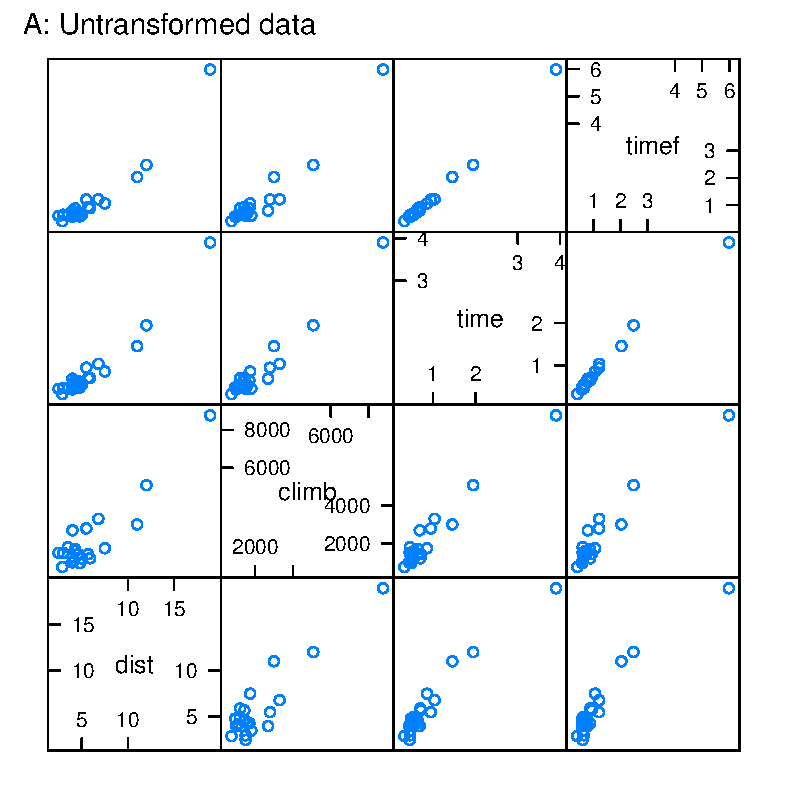
\includegraphics[width=0.48\textwidth]{figs/03-nihills-spmAB-1} 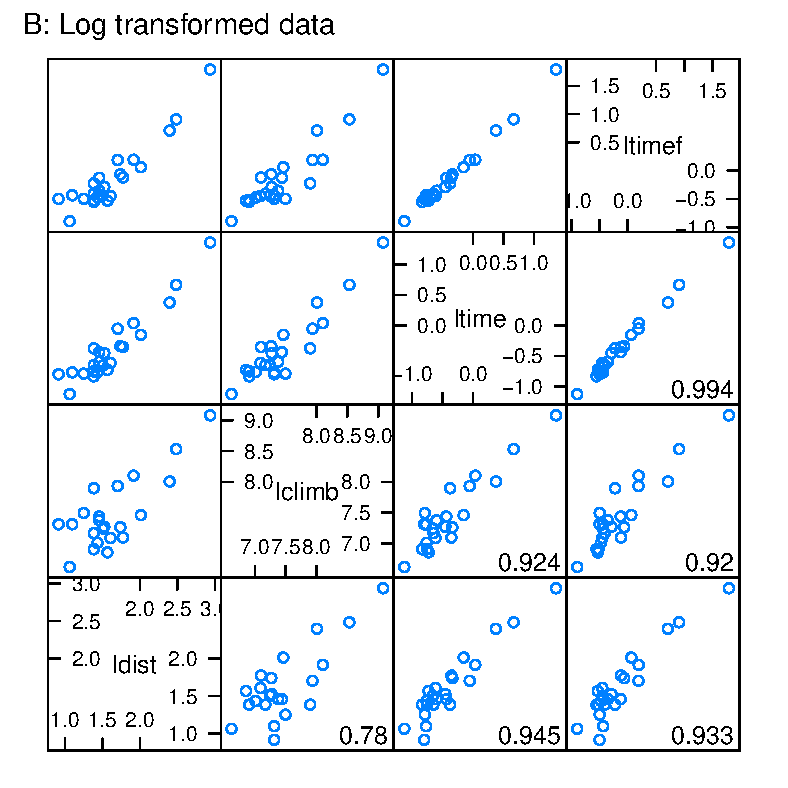
\includegraphics[width=0.48\textwidth]{figs/03-nihills-spmAB-2} }

\end{Schunk}
\caption{Scatterplot matrices for the Northern Ireland mountain racing
  data. The left panel is for the unlogged data, while the right panel is
for the logged data.  Code has been added that shows the correlations,
in the lower panel.\label{fig:nimra}}
\end{figure*}
\vspace*{15pt}

The following panel function was used to show the correlations:
\begin{Schunk}
\begin{Sinput}
showcorr <- function(x,y,...){
    panel.xyplot(x,y,...)
    xy <- current.panel.limits()
    rho <- paste(round(cor(x,y),3))
    eps <- 0.035*diff(range(y))
    panel.text(max(x), min(y)+eps, rho,
               pos=2, offset=-0.2)
}
\end{Sinput}
\end{Schunk}

Code for the scatterplot matrix in the left panel is:
\begin{Schunk}
\begin{Sinput}
## Scatterplot matrix; unlogged data
library(lattice)
splom(~nihills,  xlab="",
       main=list("A: Untransformed data", x=0,
       just="left", fontface="plain"))
\end{Sinput}
\end{Schunk}

For the right panel, create a data frame from the logged data:
\begin{Schunk}
\begin{Sinput}
lognihills <- log(nihills)
names(lognihills) <- paste0("l", names(nihills))
## Scatterplot matrix; log scales
splom(~ lognihills, lower.panel=showcorr, xlab="",
       main=list("B: Log transformed data", x=0,
       just="left", fontface="plain"))
\end{Sinput}
\end{Schunk}
%% Alternatively, give new names
%% directly:
%% <<newnames, eval=FALSE>>=
%% @ %
\marginnote[15pt]{Unlike \margtt{paste()}, the function \margtt{paste0()} does
not leave spaces between text strings that it pastes together.}

Note that the data are positively skewed, i.e., there is a long tail
to the right, for all variables. For such data, a logarithmic
transformation often gives more nearly linear relationships.  The
relationships between explanatory variables, and between the dependent
variable and explanatory variables, are closer to linear when
logarithmic scales are used.  Just as importantly, issues with large
leverage, so that the point for the largest data values has a much
greater leverage and hence much greater influence than other points on
the the fitted regression, are greatly reduced.

Notice also that the correlation of 0.913 between \txtt{climb} and
\txtt{dist} in the left panel of Figure \ref{fig:nimra} is very
different from the correlation of 0.78 between \txtt{lclimb} and
\txtt{ldist} in the right panel. Correlations where distributions are
highly skew are not comparable with correlations where distributions
are more nearly symmetric.  The statistical properties are different.


The following regresses \txtt{log(time)} on \txtt{log(climb)} and
\txtt{log(dist)}:
\begin{Schunk}
\begin{Sinput}
nihills.lm <- lm(ltime ~ lclimb + ldist,
                 data=lognihills)
\end{Sinput}
\end{Schunk}

\section{One-way Comparisons}

\marginnote[12pt]{A common strategy for getting a valid comparison is to
  grow the plants in separate pots, with a random arrangement of pots.}
The dataset \txtt{tomato} has weights of plants that were grown
under one of four different sets of experimental comditions.
Five plants were grown under each of the treatments:
\begin{itemizz}
  \item[-] \txtt{water only}
  \item[-] \txtt{conc nutrient}
  \item[-] \txtt{2-4-D + conc nutrient}
  \item[-] \txtt{x conc nutrient}
\end{itemizz}
Figure \ref{fig:Tomato}, created
using the function \txtt{quickplot()} from the {\em ggplot2} package,
shows the plant weights.  Are the apparent differences between
treatments large enough that they can be distinguished statistically?

\begin{figure}
\vspace*{-6pt}
\begin{Schunk}


\centerline{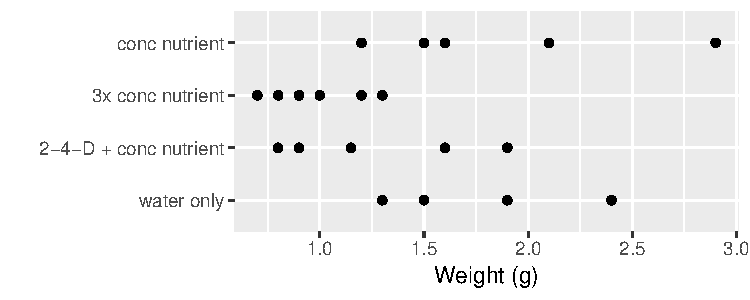
\includegraphics[width=0.98\textwidth]{figs/03-gg-tomato-1} }

\end{Schunk}
\caption{Weights (g) of tomato plants grown under four different
  treatments.\label{fig:Tomato}}
\end{figure}

\marginnote{Notice that ``water only'' is made the reference level.
This choice makes best sense for the analysis of
variance calculations that appear below.}
\begin{Schunk}
\begin{Sinput}
## Code
library(ggplot2)
tomato <- within(DAAG::tomato, 
                 trt <- relevel(trt, ref="water only"))
quickplot(weight, trt, data=tomato,
          xlab="Weight (g)", ylab="")
\end{Sinput}
\end{Schunk}

\marginnote[12pt]{Observe that, to get estimates and SEs of treatment
  effects, \margtt{tomato.aov} can be treated as an \txtt{lm} (regression)
  object.}
The command \txtt{aov()}, followed by a call to \txtt{summary.lm()},
can be used to analyse these data, thus:
\begin{Schunk}
\begin{Sinput}
tomato.aov <- aov(weight ~ trt, data=tomato)
round(coef(summary.lm(tomato.aov)), 3)
\end{Sinput}
\end{Schunk}
\begin{fullwidth}

\begin{Schunk}
\begin{Soutput}
                         Estimate Std. Error t value Pr(>|t|)
(Intercept)                 1.683      0.187   9.019    0.000
trt2-4-D + conc nutrient   -0.358      0.264  -1.358    0.190
trt3x conc nutrient        -0.700      0.264  -2.652    0.015
trtconc nutrient            0.067      0.264   0.253    0.803
\end{Soutput}
\end{Schunk}

\end{fullwidth}
Because we made ``\txtt{water only}'' the reference level,
``\txtt{(Intercept)}'' is the mean for \txtt{water only}, and the
other coefficients are for differences from \txtt{water only}.

\subsection*{A randomized block comparison}

Growing conditions in a glasshouse or growth chamber ---
temperature, humidity and air movement --- will not be totally
uniform. This makes it desirable to do several repeats of the
comparison between treatments\sidenote{In language used
originally in connection with agricultural field trials,
where the comparison was repeated on different blocks of land,
each different location  is a "block".}, with conditions
within each repeat  ("block") kept as uniform as possible.
Each different "block" may for example be a different part of
the glasshouse or growth chamber.

The dataset \txtt{DAAG::rice} is from an experiment
where there were six treatment combinations ---
three types of fertilizer were applied to each of two varieties
of rice plant.  There were two repeats, i.e., two blocks.

\begin{figure}
\begin{Schunk}


\centerline{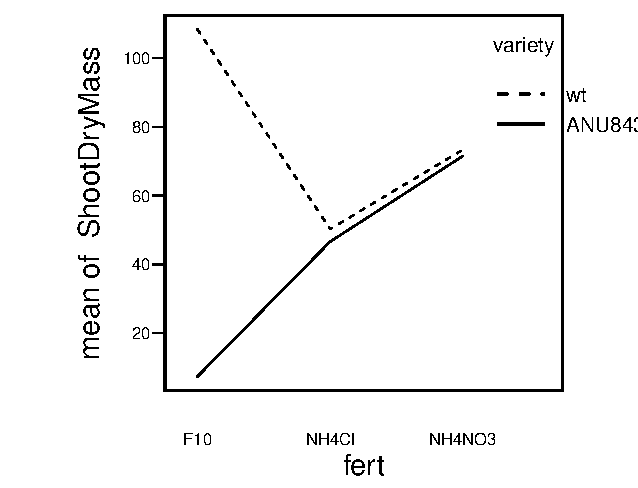
\includegraphics[width=0.65\textwidth]{figs/03-do-interact-1} }

\end{Schunk}
    \caption{Interaction plot for the terms \txtt{fert} and
      \txtt{variety}, with \txtt{ShootDryMass} as the dependent
      variable. Notice that for fertilizer F10, there is a huge
      variety difference in the response. For the other fertilizers,
      there is no difference of consequence.\label{fig:rice-interact}}
\begin{Schunk}
\begin{Sinput}
## Code
library(DAAG)
with(rice, interaction.plot(x.factor=fert,
                            trace.factor=variety,
                            ShootDryMass,
                            cex.lab=1.4))
\end{Sinput}
\end{Schunk}
\end{figure}

For these data, 
\marginnote{The effect of an appropriate choice of clocks, then
carrying out an analysis that accounts for block effects, is to
allow a more precise comparison between treatments.}
Figure \ref{fig:rice-interact} gives a clear picture
of the result. For fertilizers \txtt{NH4Cl} and \txtt{NH4NO3}, any
difference between the varieties is inconsequential.   There is
strong ``interaction'' between \txtt{fert} and \txtt{variety}.  A
formal analysis, accounting for block differences, will confirm what
seems already rather clear. 

\section{Time series -- Australian annual climate data}
\marginnote{Data
  are from the website\\
  \url{http://www.bom.gov.au/climate/change/}}

The data frame \txtt{bomregions2012} from the {\em DAAG} package has
annual rainfall data, both an Australian average and broken down by
location within Australia, for 1900 -- 2012.
Figure \ref{fig:mdbRain} shows annual rainfall in the Murray-Darling
basin, plotted against year.

\begin{figure}
\begin{Schunk}


\centerline{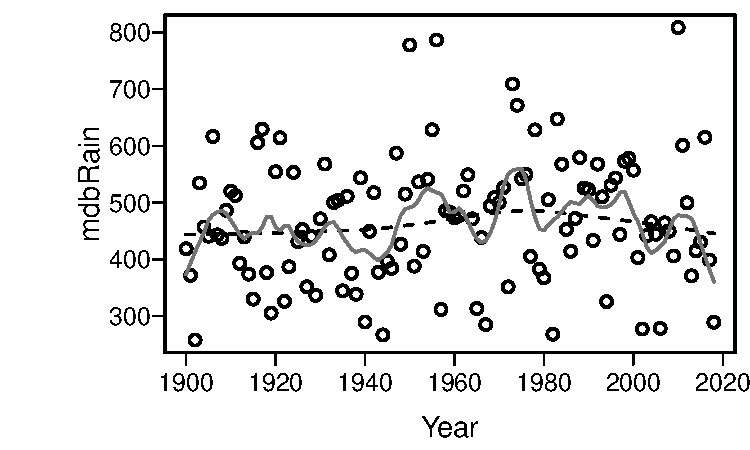
\includegraphics[width=0.98\textwidth]{figs/03-MDBrainfall-1} }

\end{Schunk}
\caption{Annual rainfall in the Australian Murray-Darling Basin.
by year.  The \txtt{lowess()} function is used to
The dashed curve with \txtt{f=2/3} captures the
overall trend, while the solid curve with \txtt{f=0.1}
captures trends on a scale of around eleven years. (10\% of the 113 year
range from 1900 to 2012 is a little more than 11 years.)\label{fig:mdbRain}}
\vspace*{-6pt}
\end{figure}

\begin{fullwidth}

\begin{Schunk}
\begin{Sinput}
## Code
library(DAAG)
plot(mdbRain ~ Year, data=bomregions2012)
## Calculate and plot curve showing long-term trend
with(bomregions2012, lines(lowess(mdbRain ~ Year, f=2/3), lty=2))
## Calculate and plot curve of short-term trends
with(bomregions2012, lines(lowess(mdbRain ~ Year, f=0.1),
                           lty=1, col="gray45"))
\end{Sinput}
\end{Schunk}

\end{fullwidth}

\marginnote[12pt]{For each smoothing window, a line or other simple
  response function is fitted. Greatest weight to points near the centre of the
  smoothing window, with weights tailing off to zero at the window edge.}
The \txtt{lowess()} function has been used to fit smooth curves,
formed by moving a smoothing window across the data.
The dashed curve with \txtt{f=2/3} (include 2/3 of the data in the
smoothing window) captures the overall trend in the data.
The choice of \txtt{f=0.1} for the solid curve has the effect that
somewhat more than ten years of data are used in determining each
fitted value on the smooth.

\marginnote[12pt]{The functions
\txtt{acf()} and \txtt{pacf()} might be used to examine the correlation
structure in the residuals.}
This graph is exploratory.  A next step might to model a
correlation structure in residuals from the overall trend.  There
are extensive abilities for this.  For graphical exploration, note
\txtt{lag.plot()} (plot series against lagged series).

The cube root of average rainfall has a more symmetric distribution
than rainfall.  Thus, use this in preference to average rainfall when
fitting models.


\section{Exercises}

% latex table generated in R 2.0.0 by xtable 1.2-2 package

\begin{enumerate}

\item Plot \txtt{Time} against \txtt{Distance}, for the
  \txtt{worldRecords} data.  Ignoring the obvious curvature, fit a
  straight line model. Use \txtt{plot.lm} to obtain diagnostic
  plots.  What do you notice?
\item The data set \txtt{LakeHuron} (\textit{datasets} package) has
  mean July average water surface elevations (ft) for Lake Huron, for
  1875-1972. The following reates a data frame that has the
  same information:
\begin{Schunk}
\begin{Sinput}
Year=as(time(LakeHuron), "vector")
huron <- data.frame(year=Year, mean.height=LakeHuron)
\end{Sinput}
\end{Schunk}
\begin{enumerate}
\item Plot \txtt{mean.height} against year.

\marginnote[12pt]{This plots the level in each year against the
level in the previous year.}
\item To see how each year's mean level is related
to the previous year's mean level, use
\begin{Schunk}
\begin{Sinput}
lag.plot(huron$mean.height)
\end{Sinput}
\end{Schunk}
%$

\item *Use the function \txtt{acf()} to plot the autocorrelation
\marginnote{For an explanation of the autocorrelation function, look up
``Autocorrelation'' on Wikepedia.}
function.  Compare with the result from the \txtt{pacf()} (partial
autocorrelation).  What do the graphs suggest?
\end{enumerate}
\end{enumerate}
